\chapter{NumPy}

\section{Introduzione}

Numpy è un modulo fondamentale per il calcolo scientifico, permette di lavorare in maniera molto efficiente su una mole di dati, ad esempio di tipo vettoriale, molto grande. Le strutture dati python sono molto interessanti, però per effettuare calcoli complessi è consigliato sfruttare numPy, dal momento che è scritto in c, c++.\\
NumPy arricchisce python con l'array-multidimensionale e aggiunge utili funzioni matematiche di base.

\section{Vantaggi}

\begin{itemize}
	\item le funzioni agiscono a livello vettoriale, questo è vantaggioso, in quanto poche volte si ricorre all'utilizzo di loop espliciti (che sono più lenti);
	\item codice scritto in c, c++, dunque è molto efficiente;
	\item gli algoritmi sono ben testati e progettati (perchè la libreria è molto utilizzata);
	\item mentre in python le strutture dati possono contenere oggetti qualsiasi, in numPy non è possibile;
\end{itemize}

\section{OpenCV e numPy}

Numpy è fondamentale perchè fa da wrapper per OpenCV, permette di sfruttarne tutte le possibilità. Il trasferimento di dati in OpenCV avviene grazie a numPy in maniera molto efficiente.

\section{La classe ndarray}

Tutti gli array numPy sono oggetti di questo tipo, implementa un array multidimensionale omogeneo (tutti gli elementi hanno lo stesso tipo). Gli attributi importanti sono:
\begin{itemize}
	\item ndim: Il numero di dimensioni;
	\item shape: tupla che indica il numero di elementi lungo ciascuna dimensione
	\item size: numero totale di elementi dell'array
	\item dtype: tipo degli elementi
	\item itemsize: dimensione in byte di ogni elemento
	\item data: il buffer contenente gli elementi (normalmente non serve: si accede agli elementi con le parentesi quadre)
\end{itemize}

\begin{lstlisting}
	#Da una lista di liste python il costruttore numpy.array capisce che noi vogliamo creare un array multidimensionale, a conterra' un riferimento all'oggetto numpy creato
	
	a = np.array([[ 0, 1, 1, 2, 3],
					[ 5, 8, 13, 21, 34],
					[ 55, 89, 144, 233, 377]])

	print('type:', type(a)) #type:
	print('ndim:', a.ndim) #ndim: 2
	print('shape:', a.shape) #(3, 5)
	print('size:', a.size) #15
	print('dtype:', a.dtype) #int32
	print('itemsize:', a.itemsize)#4
\end{lstlisting}

\section{Creare un array numpy}

\subsection{la funzione array}

\begin{lstlisting}
	# La funzione array consente di creare un array partendo da una lista o tupla Python
	# Il tipo dell'array viene dedotto dagli elementi, oppure puo' essere specificato
	a = np.array([2,3,5])
	print(a.ndim, a.shape, a.dtype, a.itemsize) #1 (3,) int32 4
	
	a = np.array([2,3,5], np.uint8)
	print(a.ndim, a.shape, a.dtype, a.itemsize) #1 (3,) uint8 1
	
	# Sequenze di sequenze sono trasformate in array bidimensionali,
	# sequenze di sequenze di sequenze in array tridimensionali e cosi' via
	a = np.array([[ 0, 1, 1, 2, 3],
						[ 5, 8, 13, 21, 34],
						[ 55, 89, 144, 233, 377]])
	print(a.ndim, a.shape, a.dtype, a.itemsize) #2 (3,5) int32 4
	a = np.array([ [ [1,2] ], [ [3,4] ] ]) #lista di liste di liste 
	print(a.ndim, a.shape, a.dtype, a.itemsize)
#3 (2, 1, 2) int32 4
\end{lstlisting}

\newpage

\subsection{Altri modi per costruire un array}

\begin{lstlisting}
	# empty() crea un array lasciando i valori non inizializzati, come si puo' osservare, attraverso una tupla impongo la dimensione del mio array, posso eventualmente aggiungere, come secondo argomento, il tipo di dato.
	a = np.empty((2,7), np.int16) # 2 righe, 7 colonne
	print(a)
	
	# zeros() e ones(): valori a zero/uno
	print(np.zeros(5)) #posso passargli un singolo valore o una tupla, per indicare la dimensione
	print(np.ones(3, np.int))
	print(np.zeros((2,3)))
	
	#arange() e' simile a range() di Python
	a = np.arange(100, 110, 2)
	print(a)
	#identity() crea una matrice identita'
	a = np.identity(3)
	print(a)

	
	#Output
	[[ -4352 26016 546 0 4 0 1]
	[ 29184 -16960 25809 546 0 -16992 25809]]
	
	[0. 0. 0. 0. 0.]
	[1 1 1]
	[[0. 0. 0.]
	[0. 0. 0.]]
	
	[100 102 104 106 108]
	
	[[1. 0. 0.]
	[0. 1. 0.]
	[0. 0. 1.]]
\end{lstlisting}

\newpage

\section{Operazioni di base}

\begin{lstlisting}
	# Gli operatori aritmetici si applicano agli array elemento-per-elemento:
	# il risultato viene tipicamente memorizzato in un nuovo array
	a = np.array( [25,36,49,64] )
	b = np.arange( 4 ) #specificando solo un valore si intende da 0 fino a 4 escluso, funziona come range 
	print(b)

	#Tutte le operazioni fra array numpy sono eseguite elemento per elemento, infatti, per calcolare c, e' necessario che a e b abbiano la stessa dimensione.
	c = a-b
	print(c)

	print(b**2) #eleva a potenza un array numpy, elemento per elemento.

	print(np.sqrt(a)) #questo e' il primo esempio di ufunc(), ovvero universal function, posso passargli un array numpy.

	# I confronti seguenti producono array di
	# valori booleani con le stesse dimensioni di a
	print(a < 37) #scrivere che una matrice a e' minore di 37, significa confrontare elemento per elemento, verificando che tutti i componenti dell'array siano minori di 37.

	b = np.array( [25,37,49,63] )
	print(a == b)	#e' un array di booleani, confronta elemento per elemento i due array, e inserisce true se sono uguali e false altrimenti. ATTENZIONE: non sta controllando se a e b sono due array numericamente uguali, per fare cio' occorre usare np.equals(a, b)
	
.	#Output

	[0 1 2 3]

	[25 35 47 61]

	[0 1 4 9]

	[5. 6. 7. 8.]
	
	[ True True False False]
	
	[ True False True False]
\end{lstlisting}

\newpage

\section{Operazione prodotto}

\begin{lstlisting}
	# Anche l'operatore prodotto '*' opera elemento-per-elemento;
	# Dalla v3.5 di Python e' disponibile l'operatore '@' per i prodotti fra matrici
	A = np.array( [[1,1],
						[0,1]] )
	B = np.array( [[2,0],
						[3,4]] )
	
	print(A * B) # Prodotto elemento-per-elemento:(1*2 = 2; 1*0 = 0; 0*3 = 0; 1*4 =4)
	
	print(A @ B) # Prodotto tra matrici (riga * colonna, faccio la prima riga di A * prima colonna di B e cosi' via), molto elegante
	
	# Un vettore "colonna": shape = (3, 1)
	c = np.array([[1], [2], [3]])
	# Un vettore "riga": shape = (1, 3)
	r = np.array([[3,0,2]])
	
	print(c @ r) # (3,1)x(1,3) = (3,3)
	
	print(r @ c) # (1,3)x(3,1) = (1,1)

	
	#Output
	[[2 0]
	[0 4]]

	[[5 4]
	[3 4]]

	[[3 0 2]
	[6 0 4]
	[9 0 6]]

	[[9]]
	
\end{lstlisting}
\newpage

\section{Operatori di assegnamento}


\begin{lstlisting}
	# Gli operatori di assegnamento come += o *= modificano
	# l'array esistente senza doverne creare uno nuovo
	
	a = np.ones((2,3))
	b = np.array([[1,0,2], [0,3,0]])
	
	id_a = id(a)
	
	a *= b #viene modificato il contenuto di a senza che venga riallocato un altro oggetto, basti ricordare che le liste sono modificabili
	
	print(a)
	
	print(id_a, id(a), id_a==id(a))
	
	a = a * b
	
	print(a)
	
	print(id_a, id(a), id_a==id(a))
	
	#Output
	
	[[1. 0. 2.]
	[0. 3. 0.]]
	
	2346790588544 2346790588544 True
	
	[[1. 0. 4.]
	[0. 9. 0.]]
	
	2346790588544 2346791113632 False
\end{lstlisting}

\newpage

\section{Type cast}

\begin{lstlisting}
	a = np.ones(3, np.int32)
	b = np.array([1.4, 1.5, 1.6])
	print(a.dtype, b.dtype)
	# In una operazione fra array di tipo diverso,
	# il tipo del risultato corrisponde a quello piu'
	# preciso (o piu' generale) dei due
	c = a + b
	print(c)
	print(c.dtype)
	# Per creare un nuovo array cambiando il tipo di un
	# array esistente, si puo' usare il metodo astype()
	a = np.arange(10, dtype = np.uint8)
	print(a.dtype)
	a = a.astype(np.uint64)
	print(a.dtype)

	
	#Output
	
	int32 float64
	
	[2.4 2.5 2.6]
	
	float64
	
	uint8
	
	uint64
	
\end{lstlisting}

\section{Alcune operazione su un array}

\begin{lstlisting}
	#Crea una matrice contenente numeri casuali nell'intervallo [0,1)

	a = np.random.random((2,3))
	print(a)
	
	# Calcola il valore minimo, massimo e la somma
	print(f'Min: {a.min()}')
	print(f'Max: {a.max()}')
	print(f'Sum: {a.sum()}')
	
	# Il calcolo, invece che su tutti gli elementi,
	# puo' essere lungo uno specifico asse
	
	print(f'Somma di ogni colonna: {a.sum(axis=0)}')
	print(f'Somma di ogni riga: {a.sum(axis=1)}')

\end{lstlisting}

\section{Funzioni universali (ufunc)}

Funzioni numpy che operano su ndarray elemento-per-elemento. Alcuni esempi:
\begin{itemize}
	\item Operazioni matematiche;
	\item Trigonometria;
	\item Operazioni sui bit;
	\item Confronto;
	\item Floating point.
\end{itemize}



\section{Indicizzazione e slicing su array monodimensionali}

\begin{lstlisting}
	# Negli array NumPy monodimensionali, l'accesso agli elementi e' analogo a
	# quanto avviene con liste e altre sequenze in Python
	a = np.arange(10)**3 #10 elementi e ogni singolo elemento lo elevo al cubo
	print(a)
	print(a[2]) # Accesso a un elemento
	print(a[2:5]) # Slicing: dall'elemento 2 al 4
	a[:6:2] = 42 # Modifica elementi di posto 0, 2, 4
	print(a)
	print(a[::-1]) # Step negativo: ordine inverso
	a[::2] += a[1::2] # a[i] += a[i+1], i=0,2,4,6,8
	print(a)
	a[:] = -1 # Modifica tutti gli elementi
	print(a)

	
	#Output
	
	[ 0 1 8 27 64 125 216 343 512 729]
	
	8
	
	[ 8 27 64]
	
	[ 42 1 42 27 42 125 216 343 512 729]
	
	[729 512 343 216 125 42 27 42 1 42]
	
	[ 43 1 69 27 167 125 559 343 1241 729]
	
	[-1 -1 -1 -1 -1 -1 -1 -1 -1 -1]
\end{lstlisting}

\newpage

\section{Indicizzazione e slicing su array multidimensionali}

La funzione fronmfunction è molto utile, permette di passare una funzione python (che prende come parametri due interi, perchè ci sono due dimensioni) e sulla base della funzione crea un array multidimensionale delle dimensioni definite e con valori ottenuti applicando la funzione.

\begin{figure}[ht]
	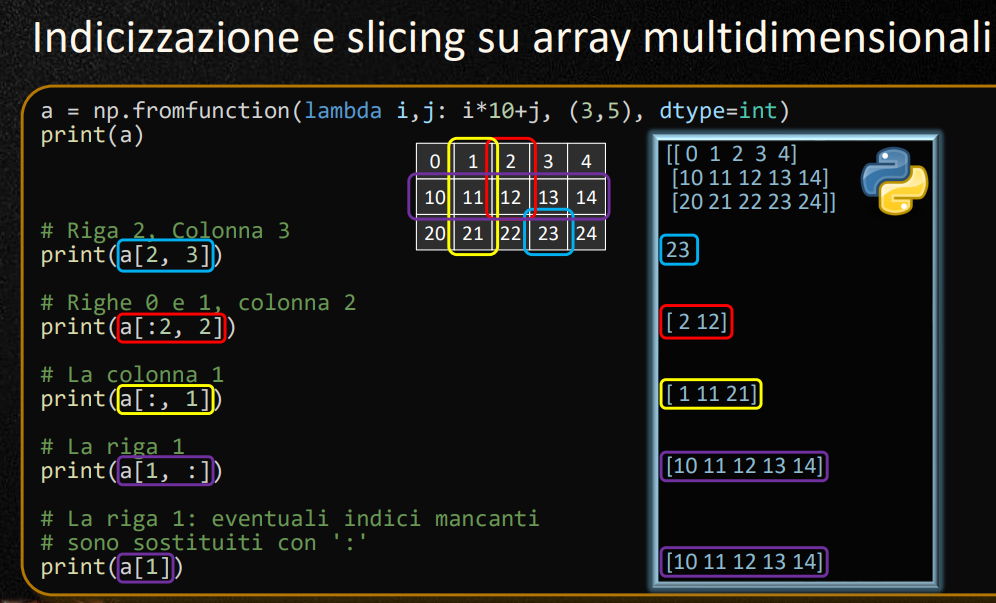
\includegraphics[width=450pt]{./immagini/slicing_array_multidimensionali.png}
	\label{img:slicing_array_multidimensionali}
\end{figure}

Nello slicing di matrici, se ometto il secondo termine, facendo ad esempio a[1:3] è come se sottointendessi a[1:3,:], quindi righe da 1 a 3 poi tutte le colonne.

\begin{figure}[htt]
	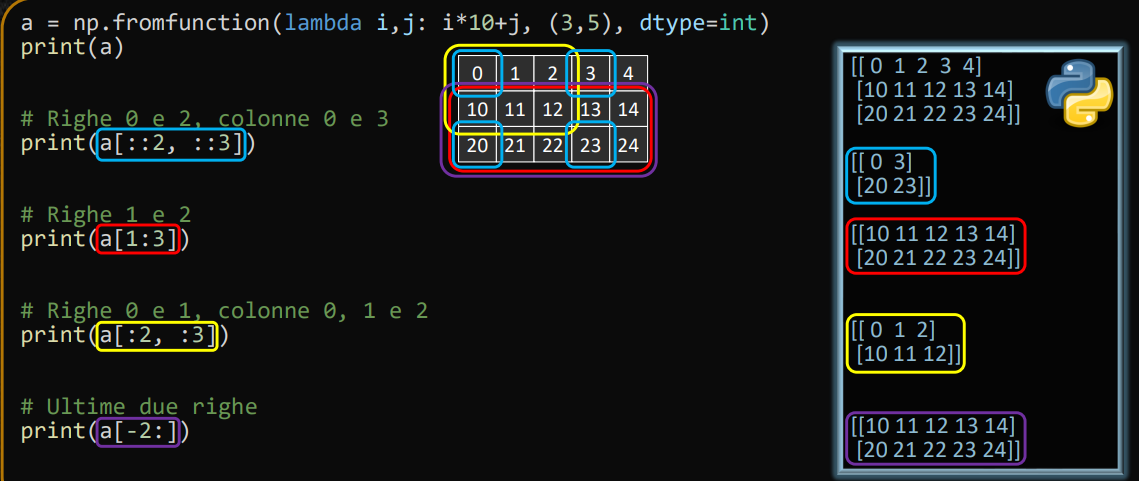
\includegraphics[width=500pt]{./immagini/slicing_array_multidimensionali1.png}
	\label{img:slicing_array_multidimensionali1}
\end{figure}

\newpage

\section{Iterare un array}

Di solito non si fanno iterazioni usando numpy, si riesce quasi sempre a trasformare dei cicli in funzioni vettoriali. Nonostante cio' puo' capitare di iterare.

\begin{lstlisting}
	a = np.arange(7)
	print(a)
	# Si puo' iterare sugli elementi un array monodimensionale

	for x in a:
		print(x, end='; ')
	print()
	
	a = np.fromfunction(lambda i,j: i*10+j, (3,5), dtype=int)
	print(a)
	
	# Iterando su una matrice si ottengono le righe...
	for r in a:
		for x in r: # ... su cui si puo' ulteriormente iterare
			print(x, end='; ')
		print()
	# L'attributo .flat e' un iteratore su tutti gli elementi
	for x in a.flat:
		print(x, end=', ')

	
	#Output
	
	[ 0 1 8 27 64 125 216 343 512 729]
	
	8
	
	[ 8 27 64]
	
	[ 42 1 42 27 42 125 216 343 512 729]
	
	[729 512 343 216 125 42 27 42 1 42]
	
	[ 43 1 69 27 167 125 559 343 1241 729]
	
	[-1 -1 -1 -1 -1 -1 -1 -1 -1 -1]
\end{lstlisting}

\newpage

\section{Slicing con ellissi}

Utile quando ho un array con molti assi (3 dimensioni o più), i puntini ci evitano di dover precisare tutte le dimnesioni.

\begin{figure}[htp]
	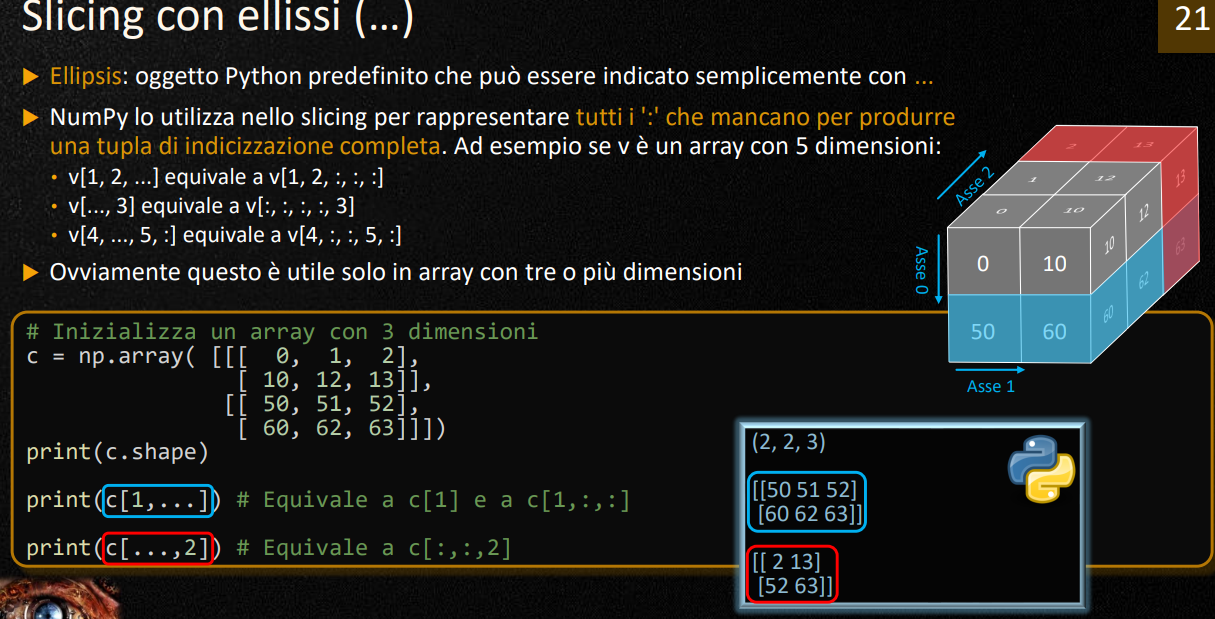
\includegraphics[width=500pt]{./immagini/slicing_array_multidimensionali2.png}
	\caption{Esempio di periodo}
	\label{img:slicing_array_multidimensionali2}
\end{figure}

\section{Modifica della forma}

Differenza reshape e resize : reshape costruisce un nuovo array e lo restituisce, resize non restituisce nulla, modifica l'array sulla quale viene chiamato il metodo.

\begin{lstlisting}
	a = np.arange(12)
	print(a.shape)
	print(a)

	# reshape() restituisce gli stessi con forma diversa
	b = a.reshape(2, 6)
	print(b.shape)
	print(b)

	# Se una dimensione e' -1, viene calcolata automaticamente
	c = a.reshape(2, 2, -1)
	print(c.shape)
	print(c)

	a.resize(2,6) # resize() modifica l'array stesso
	print(a)

	# ravel() restituisce i dati come array monodimensionale
	d = a.ravel()
	print(d)

	
	
	#Output
	
	(12,)
	[ 0 1 2 3 4 5 6 7 8 9 10 11]
	(2, 6)
	[[ 0 1 2 3 4 5]
	[ 6 7 8 9 10 11]]
	(2, 2, 3)
	[[[ 0 1 2]
	[ 3 4 5]]
	[[ 6 7 8]
	[ 9 10 11]]]
	[[ 0 1 2 3 4 5]
	[ 6 7 8 9 10 11]]
	[ 0 1 2 3 4 5 6 7 8 9 10 11]
	
\end{lstlisting}

\subsection{Altri modi per modificare la forma}

C'è la possibilità di aggiungere nuove dimensioni con cardinalità uno con np.newaxis.

\begin{lstlisting}
	a = np.arange(12).reshape(2,6)
	print(a)
	
	# Aggiunta di nuove dimensioni con np.newaxis
	b = a[np.newaxis, ...] #Aggiungo alla shape di a un nuovo asse, serve se mi occorre operare su un array di dimensione diversa rispetto a quella attuale
	print(b.shape)
	print(b)
	c = a[np.newaxis, ..., np.newaxis, np.newaxis]
	print(c.shape)
	
	# np.newaxis non e' altro che un riferimento a None
	print(np.newaxis is None)
	
	# Scambiare le dimensioni con transpose() o .T
	d = a.T
	e = a.transpose()
	print(d.shape, e.shape)
	
	# squeeze() elimina eventuali dimensioni a uno, torna utile nel caso in cui mi serve togliere le dimensioni in piu'.
	f = c.squeeze()
	print(f.shape)
	
	
	#Output
	
	(12,)
	[ 0 1 2 3 4 5 6 7 8 9 10 11]
	(2, 6)
	[[ 0 1 2 3 4 5]
	[ 6 7 8 9 10 11]]
	(2, 2, 3)
	[[[ 0 1 2]
	[ 3 4 5]]
	[[ 6 7 8]
	[ 9 10 11]]]
	[[ 0 1 2 3 4 5]
	[ 6 7 8 9 10 11]]
	[ 0 1 2 3 4 5 6 7 8 9 10 11]
	
\end{lstlisting}

\section{Concatenare array}

\begin{lstlisting}
	#Qui ha creato una matrice quadrata random di dimensione 2, moltiplicando ogni elemento per due. Con np.floor poi ha effettuato il troncamento sui numeri.
	
	a = b = np.floor(10*np.random.random((2,2)))
	print(a)
	
	print( np.vstack((a,b)) )	#vstack : vertical stack, mette in pila in verticale
	
	print( np.hstack((a,b)) )	#hstack : horizontal stack
	
	# column_stack() affianca array 1D come colonne
	# di un array 2D 
	#Ho due array monodimensionali che vengono considerati vettori colonna e vengono affiancati, e' evidente la differenza con vstack.
	x = np.array([4.,2.])
	y = np.array([3.,8.])
	print( np.column_stack((x,y)) )
	#notare la differenza se invece di usa hstack()
	print( np.hstack((x,y)) )
	#Output
	[[5. 6.]
	[2. 0.]]
	
	[[4. 8.]
	[1. 7.]]
	
	[[5. 6.]
	[2. 0.]
	[4. 8.]
	[1. 7.]]
	
	[[5. 6. 4. 8.]
	[2. 0. 1. 7.]]
	
	[[4. 3.]
	[2. 8.]]
	
	[4. 2. 3. 8.]
	
\end{lstlisting}

\section{Copie e viste di array}

Tante operazioni in numpy non producono un nuovo array con una copia dei dati, producono un nuovo oggetto ma i dati che contiene questo oggetto array sono gli stessi. Noi sappiamo che l'assegnamento non crea un nuovo oggetto ma copia solamente il riferimento. Nemmeno lo slicing non crea nuovi oggetti, è un concetto chiave di python, cambia i riferimenti.

\begin{lstlisting}
	a = np.arange(7)
	print(a)
	
	# Come per qualsiasi variabile Python, l'assegnamento
	# non crea un nuovo oggetto, solo un nuovo riferimento
	b = a
	print(b is a)
	
	# Lo slicing (come altre operazioni) crea una vista: un
	# nuovo oggetto che condivide gli stessi dati. a.base
	# e' un riferimento all'oggetto su cui e' costruita la vista
	c = a[3::2]
	print(c is a, c.base is a) #L'attributo base di un oggetto numpy e' None se contiene i propri dati e non e' la lista di un altro oggetto, se invece e' diverso da None e' una lista che contiene i propri dati. Numpy tenta di eliminare le duplicazioni inutili.
	print(c)
	c[0] = -1
	print(a) #Da questa print capiamo che sono oggetti diversi ma i dati sono gli stessi! Modificando i dati di c vengono di conseguenza modificati quelli di a. Quindi occorre ricordare che quando estraiamo gli elementi con lo slicing, in realta' otteniamo una lista sugli stessi dati... ma come faccio ad evitarlo? con il metodo copy()
	
	d = a.copy() # Il metodo copy() crea una copia dell'array
	print(d is a, d.base is a, d.base)
	d[0] = -1
	print(d, a)
	
	#Output
	
	
	[0 1 2 3 4 5 6]
	
	True
	
	False True
	
	[3 5]
	
	[ 0 1 2 -1 4 5 6]
	
	False False None
	
	[-1 1 2 -1 4 5 6] [ 0 1 2 -1 4 5 6]
\end{lstlisting}

\newpage

\section{Broadcasting}

\begin{figure}[htp]
	\includegraphics[width=500pt]{./immagini/Broadcasting.png}
	\caption{Esempio di periodo}
	\label{img:Broadcasting}
\end{figure}

\section{Indicizzare con un array di indici}

\begin{lstlisting}
	a = np.arange(12)**2
	print(a)
	# Oltre a interi e slicing, si possono
	# utilizzare array di interi per
	# indicizzare altri array
	idx1 = np.array( [ 1,1,3,8,5 ] )
	print(a[idx1])
	# L'array di interi puo' anche
	# essere multidimensionale: il
	# risultato ha la forma dell'array
	# usato come indice
	idx2 = np.array( [ [3, 4], [9, 7] ] )
	print(a[idx2])

	
	#Output
	
	[ 0 1 4 9 16 25 36 49 64 81 100 121]
	
	[ 1 1 9 64 25]
	
	[[ 9 16]
	[81 49]]
\end{lstlisting}

\section{Indicizzare un array multidimensionale con un array di indici}

\begin{lstlisting}
	# Se l'array a e' multidimensionale si puo' passare un array
	# di indici per ciascuna dimensione, purche' abbiamo la stessa
	# forma (o si possa fare broadcast fra loro).
	# Come per lo slicing, si puo' utilizzare ':' o '...'
	# per non dover specificare tutte le dimensioni.
	a = (np.arange(12)**2).reshape(3,4)
	print(a)
	
	idx2 = np.array([1,1,2])
	print(a[idx2,:]) # oppure print(a[idx2])
	print(a[:,idx2])
	
	idx_r = np.array( [ [0,0,0], [1,1,1] ] )
	idx_c = np.array( [ [2,3,2], [0,0,0] ] )
	print(a[idx_r,idx_c])

	
	#Output
	
	[[ 0 1 4 9]
	[ 16 25 36 49]
	[ 64 81 100 121]]
	
	[[ 16 25 36 49]
	[ 16 25 36 49]
	[ 64 81 100 121]]
	
	[[ 1 1 4]
	[ 25 25 36]
	[ 81 81 100]]
	
	[[ 4 9 4]
	[16 16 16]]
\end{lstlisting}

\newpage

\section{Indicizzare con array di booleani}

\begin{lstlisting}
	# Nell'indicizzazione con array di interi si specificano
	# gli indici da considerare, invece in questo caso si scelgono
	# esplicitamente quali elementi si vogliono e quali no.
	# Il modo piu' semplice e' utilizzare array booleani con la
	# stessa forma dell'array originale.
	a = np.arange(12).reshape(3,4)
	print(a)
	
	b = a > 4
	print(b) # array booleano con la stessa forma di a
	
	print(a[b]) # un array 1D con gli elementi considerati
	
	# La selezione con elementi booleani e' molto utile per
	# modificare solo gli elementi che soddisfano un certo criterio.
	criterio = a%3 == 0
	print(criterio)
	
	print(a[criterio])

	
	#Output
	
	[[ 0 1 2 3]
	[ 4 5 6 7]
	[ 8 9 10 11]]

	[[False False False False]
	[False True True True]
	[ True True True True]]

	[ 5 6 7 8 9 10 11]

	[[ True False False True]
	[False False True False]
	[False True False False]]

	[0 3 6 9]
\end{lstlisting}